\begin{answer}

The last feature $sin(x)$ donimates other features. With k increasing, the improvement of fitting is limited. So it no longer requires a relatively high degree k to fit the given training data

\begin{figure}
    \centering
    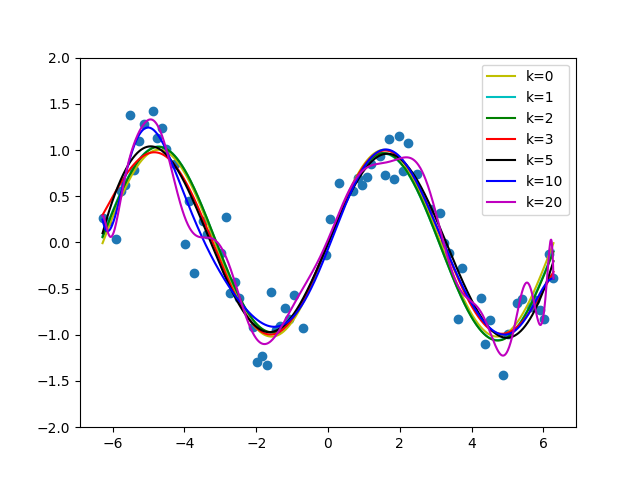
\includegraphics[width=0.5\linewidth]{ps1_q3_(d).png}
    \caption{ps1\_q3\_(d)}
    \label{fig:enter-label}
\end{figure}
\end{answer}
